\chapter{Historique des mécanismes de protection}
\label{chap:historique}

La gestion de la mémoire est un des composants le plus complexe d'un système d'exploitation moderne, ce qui rend le sujet bien plus vaste que ce que l'on peut traiter dans ce rapport. Cependant, il m'a été nécessaire de parcourir les principaux concepts pour pouvoir en comprendre les enjeux.

Dans ce chapitre, un bref récapitulatif de cette gestion est fait en préambule de la partie historique des attaques et des mécanismes de protection. Les cas expliqués dans ce rapport sont volontairement simplifiés de manière à comprendre l'aspect conceptuel et non pratique. Exploiter dans un environement réel certaines des attaques brièvement décrites par la suite peut occuper le volume d'un rapport au moins égal à celui-ci.

La description du fonctionnement de la mémoire est inspirée des articles suivants \cite{AnatomyOfAProgramInMemory, HowTheKernelManagesYourMemory, JourneyToTheStackPartI} tirés du blog de Gustavo Duarte. À des fins de simplicité, les concepts exposés sont basé sur une architecture 32 bits. Dans le cas de changements notables entre architectures, un complément spécifique en 64 bits est donné. Les termes anglais sont mentionnés une première fois lors de leurs traductions, le document utilisera ensuite la traduction française.

\minitoc

\newpage

% ---------------------------------------------------------------------------
\section{Rappel sur la gestion de la mémoire}

La mémoire d'un programe est gérée selon un schéma bien défini. Chaque processus du système d'exploitation voit sa mémoire définie dans un espace virtuel \og virtual address space \fg, l'isolant complètement du reste des processus. Ce espace est égal à 4~Go dans un système 32~bits. Dans le cas d'une architecture 64~bits, l'espace disponible n'utilise pas $2^{64}$ octets (16~Eo), mais uniquement les 48~bits les moins significatifs, et donc $2^{48}$ octets (256~To) \cite{64bitComputing,VirtualAddressSpaceDetails}. Le système d'exploitation est ensuite responsable de faire le lien entre cet espace virtuel et l'espace d'adressage physique.

\subsection{Segmentation}

La mémoire virtuelle est scindée en deux parties principales. La première, ayant les adresses mémoires allant de \mintinline{c}{0xc0000000} à \mintinline{c}{0xffffffff} (en 32 bits), est reservée, sous Linux, au noyau du système d'exploitation. La seconde, quant à elle, correspond à l'espace disponible du processus courant.

\begin{figure}[H]
	\centering
	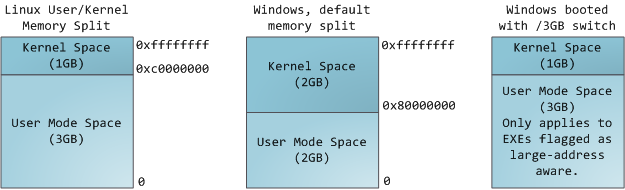
\includegraphics[width=0.8\columnwidth]{kernelUserMemorySplit}
	\captionsource{Répartition de l'espace mémoire du kernel}
	{Répartition de l'espace mémoire virtuel entre le noyau et le programme, par G.~Duarte}
	{\url{http://duartes.org/gustavo/blog/post/anatomy-of-a-program-in-memory/}}
	\label{fig:kernelUserMemorySplit}
\end{figure}

L'espace réservé au processus est ensuite découpé en différents segments tel que la pile \og stack \fg ou le tas \og heap \fg. Ces segments sont des plages mémoires continues gérées par le système d'exploitation. Dans le cas d'un processus Linux, les segments sont répartis ainsi :

\begin{figure}[H]
	\centering
	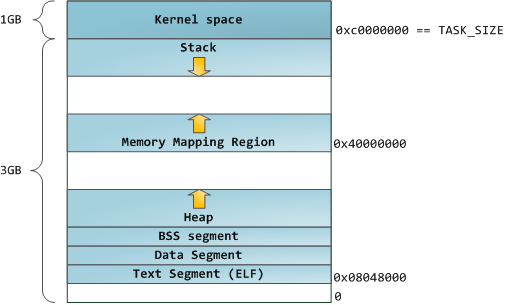
\includegraphics[width=.7\columnwidth]{linuxClassicAddressSpaceLayout}
	\captionsource{Segmentation de la mémoire d'un processus Linux 32 bits}
	{Segmentation de la mémoire d'un processus Linux en 32 bits, par G.~Duarte}
	{\url{http://duartes.org/gustavo/blog/post/anatomy-of-a-program-in-memory/}}
	\label{fig:linuxClassicAddressSpaceLayout}
\end{figure}

\vfill

La pile d'exécution permet de gérer le flot de contrôle de l'application. À chaque appel de fonction, une nouvelle structure de pile \og stack frame \fg est ajoutée à la pile, puis est retirée lorsque la fonction se termine. La pile d'exécution grandit vers le bas, c'est-à-dire que les adresses mémoires décroissent lorsque la pile se remplit. Il est possible que la pile veuille s'étendre au-delà de sa taille maximum, c'est le cas du dépassement de pile \og stack overflow \fg. Dans ce cas, le programme reçoit une erreur de segmentation, \og segmentation fault \fg en anglais, et s'arrête.

Le segment \og memory mapping region \fg permet au noyau de copier en mémoire le contenu de certains fichiers de manière à augmenter les performances. Ce segment est généralement utilisé pour charger les bilbiothèques dynamiques. Il peut aussi être utilisé à d'autres fins, par exemple pour stocker des données, tel le tas.

En dessous se trouve le tas, permettant de stocker en mémoire les allocations dynamiques. En C, ce segment est géré par la fonction \mintinline{c}|malloc()| et ses confrères. Dans d'autres langages bénéficiant d'un ramasse-miettes, tel que le C\#, l'interface pour intéragir avec le tas est le mot réservé \mintinline{c}|new|.

Finalement les trois derniers segments que sont \og BSS \fg, \og data \fg et \og text \fg servent à stocker les variables statiques initialisées ou non ainsi que la source du binaire executé. La \autoref{fig:mappingBinaryImage} illustre un exemple de ce que l'on peut retrouver dans ces segments.

\begin{figure}[H]
	\centering
	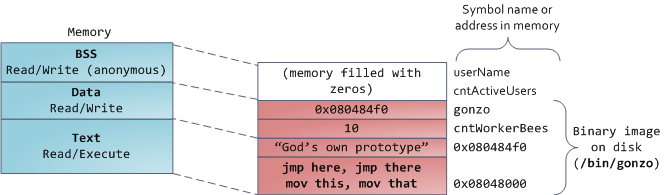
\includegraphics[width=.7\columnwidth]{mappingBinaryImage}
	\captionsource{Plan d'une image binaire dans les segments BSS, Data et Text}
	{Plan d'une image binaire dans les segments BSS, data et text, par G.~Duarte}
	{\url{http://duartes.org/gustavo/blog/post/anatomy-of-a-program-in-memory/}}
	\label{fig:mappingBinaryImage}
\end{figure}

\subsection{Descripteurs mémoires}

Lors de l'exécution d'un programme, cet espace mémoire est géré par le système d'exploitation grâce à des descripteurs de mémoire appelés \og memory descriptor \fg. Cette structure contient les adresses de début et de fin de chaque segments.

\begin{figure}[H]
	\centering
	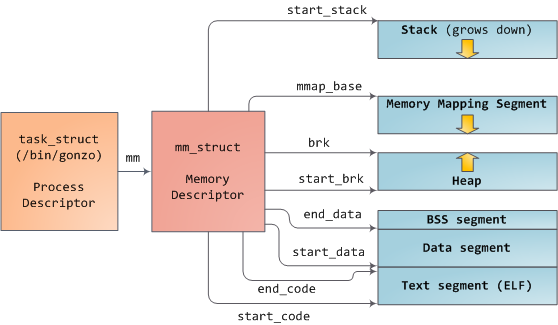
\includegraphics[width=0.5\columnwidth]{mm_struct}
	\captionsource{Descripteur de mémoire d'un processus Linux}
	{Descripteur de mémoire d'un processus Linux, par G.~Duarte}
	{\url{http://duartes.org/gustavo/blog/post/how-the-kernel-manages-your-memory/}}
	\label{fig:mm_struct}
\end{figure}

Cette structure globale est constituée d'une suite de plus petites structures appelées espaces virtuels de mémoire \og virtual memory area \fg, \mintinline{c}{vm_area_struct} sur la \autoref{fig:memoryDescriptorAndMemoryAreas}. Chacune d'elles est un espace continu en mémoire et permettent de stocker des informations tels que les droits d'écriture, de lecture ou encore les droits d'exécution du contenu mémoire. Elles stockent également si et quel fichier est mappé en mémoire.

\begin{figure}[H]
	\centering
	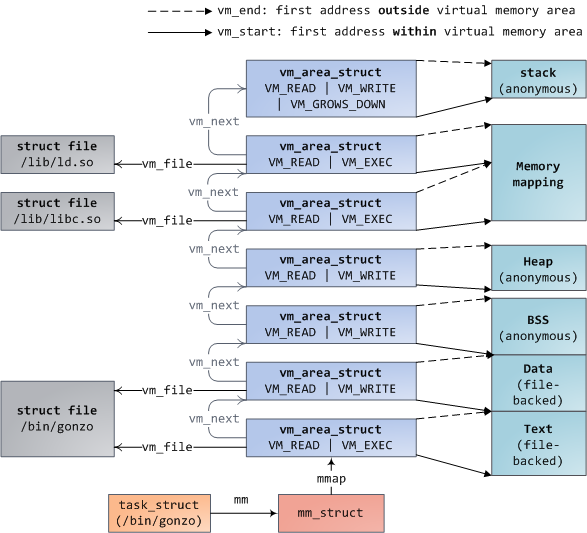
\includegraphics[width=0.7\columnwidth]{memoryDescriptorAndMemoryAreas}
	\captionsource{Structure des espaces virtuels de mémoire}
	{Structure des espaces virtuels de mémoire, par G.~Duarte}
	{\url{http://duartes.org/gustavo/blog/post/how-the-kernel-manages-your-memory/}}
	\label{fig:memoryDescriptorAndMemoryAreas}
\end{figure}

% ---------------------------------------------------------------------------
\section{\og Buffer overflow \fg}

Le dépassement de tampon, \og buffer overflow \fg en anglais, consiste à exploiter une fonction qui ne vérifie par la taille du contenu à copier en mémoire. En utilisant, par exemple, \mintinline{c}{strcpy()}, il est possible d'écrir sur l'adresse de retour de la fonction et ainsi modifier le flot de contrôle de l'application en le redirigeant à un endroit où l'attaquant aura, par exemple, préalablement injecté du code --- \og shellcode \fg \ ---.

\subsection{\og Stack frame \fg}

Une \og stack frame \fg permet de stocker toutes les informations nécessaires à l'exécution d'une fonction. Elle est créée sur la pile lors de l'appel de ladite fonction, par le prologue, et est détruite, avant l'appel de retour, par l'épilogue. Elle n'est pas détruite à proprement parlé, le pointeur \mintinline{c}{%ebp} est restauré dans son état précédent.

Lorsqu'une \og stack frame \fg est créée, celle-ci stocke dans un schéma particulier les informations dont elle a besoin. Les premières informations ont des adresses plus grandes en mémoires que les dernières, car la pile grandit de manière décroissante. La séquence suivante est exécutée à chaque prologue de fonction afin d'initialiser la \og frame \fg; sont placés sur la pile successivement:

\begin{enumerate}
	\item les paramètres passés à la fonction
	\item l'adresse de retour, équivalant à l'adresse de la fonction appelante
	\item une sauvegarde du pointeur \mintinline{c}{%ebp}, pour restaurer la \og frame \fg précédente lors de l'épilogue
	\item puis les variables locales, déclarées au sein de la fonction
\end{enumerate}

Le code d'exemple \autoref{lst:stack_example} contient une fonction \mintinline{c}{func()} qui est appelée avec deux arguments, \mintinline{c}{512} et \mintinline{c}{65536}, et qui déclare des variables locales. La \autoref{fig:stackIntro} illustre l'état de la pile à la fin de la ligne 6, avant le retour de la fonction.

\begin{listing}
	\cfile{02-main/listings/stack.c}
	\caption{Exemple de programme illustrant la gestion de la pile d'exécution}
	\label{lst:stack_example}
\end{listing}

Les deux arguments de 4~octets (en orange) sont d'abord mis sur la pile, l'adresse de retour ainsi que l'ancienne valeur de \mintinline{c}{%ebp} de 4~octets [adressage en 32~bits] (en bleu clair) sont ensuite sauvées, puis les deux variables locales, 4~octets pour l'entier et 8~octets pour le \mintinline{c}{local_buffer} (en vert à droite) sont crées.

\begin{figure}[H]
	\centering
	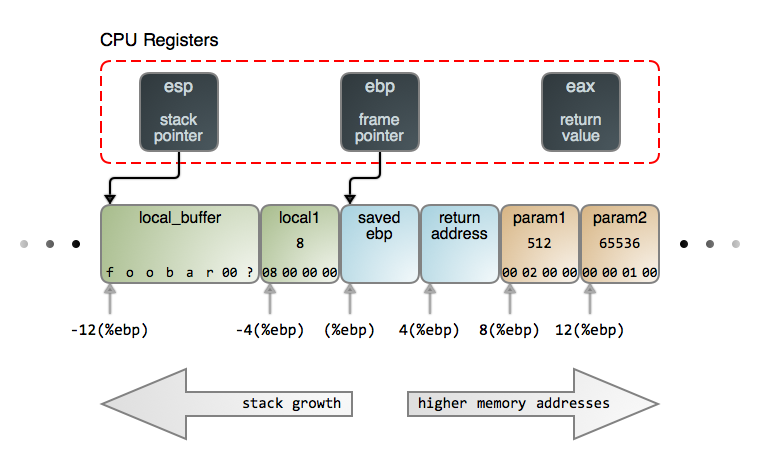
\includegraphics[width=0.6\columnwidth]{stackIntro}
	\captionsource{Exemple d'une Stack frame}
	{Exemple d'une structure de pile (Stack frame), par G.~Duarte}
	{\url{http://duartes.org/gustavo/blog/post/journey-to-the-stack/}}
	\label{fig:stackIntro}
\end{figure}

On constate alors que l'adresse de départ du \mintinline{c}{local_buffer} est inférieure de 16~octets à l'adresse stockant l'adresse de retour. Cette différence est déterministe et ne changera jamais lors de l'exécution.

\subsection{Exemple}

Grâce à cette structure, du fait que la pile grandit avec des adresses décroissantes ainsi que l'utilisation de fonction tel que \mintinline{c}{strcpy()}, il est possible, en dépassant la taille des variables locales, de modifier des zones mémoires telles que l'adresse de retour. Le code montré en \autoref{lst:buffer_example} permet d'illustrer un cas d'exploitation de la fonction \mintinline{c}{gets()} --- fonction vulnérable car elle ne s'arrête que lorsqu'elle rencontre un retour à la ligne ou un  \og \gls{eof} \fg \ ---.

\begin{listing}
	\cfile{02-main/listings/buffer.c}
	\caption{Exemple de programme illustrant un dépassement de tampon}
	\label{lst:buffer_example}
\end{listing}

En regardant la \autoref{fig:bufferCopy} on constate que si l'on écrit 28+4+4 octets = 36 octets dans le \mintinline{c}{buffer}, les 4 derniers octets auront écrasé l'adresse de retour.

\begin{figure}[H]
	\centering
	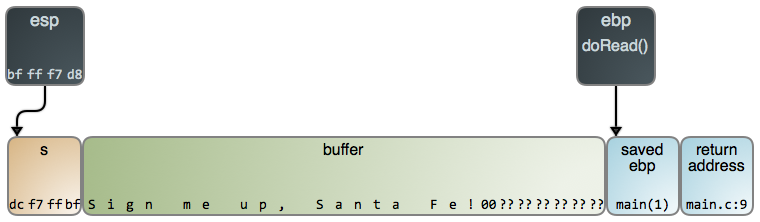
\includegraphics[width=0.8\columnwidth]{bufferCopy}
	\captionsource{Exemple de \og stack frame \fg avant un dépassement de tampon}
	{Exemple de \og stack frame \fg avant un dépassement de tampon, par G.~Duarte}
	{\url{http://duartes.org/gustavo/blog/post/epilogues-canaries-buffer-overflows/}}
	\label{fig:bufferCopy}
\end{figure}

Dans cette exemple, il est possible d'injecter un \og shellcode \fg dans le \mintinline{c}{buffer} grâce à la fonction \mintinline{c}{gets()}.

\begin{figure}[H]
	\centering
	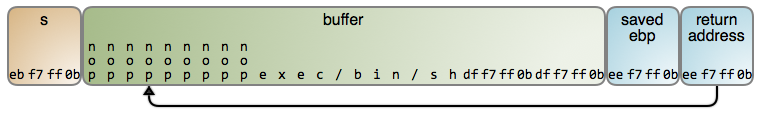
\includegraphics[width=0.8\columnwidth]{bufferOverflowExploit}
	\captionsource{Illustration de l'état de la pile au moment d'un dépassement de tampon}
	{Illustration de l'état de la pile au moment d'un dépassement de tampon, par G.~Duarte}
	{\url{http://duartes.org/gustavo/blog/post/epilogues-canaries-buffer-overflows/}}
	\label{fig:bufferOverflowExploit}
\end{figure}

\vfill

% ---------------------------------------------------------------------------
\section{DEP/NX}

Le mécanisme \gls{dep}/\gls{nx} a été mis en place pour éviter, lors d'un dépassement de tampon, que l'attaquant puisse exécuter du code stocké sur la pile. Les endroits mémoire censés contenir des données sont, via les \mintinline{c}{vm_area_struct} sous Linux, marquées comme étant non-exécutable. Le marquage indique ensuite au processeur, via le drapeau \gls{nx}, qu'il ne doit pas exécuter le contenu de cette plage mémoire.

\subsection{Mécanisme de protection}

Le mécanisme de Data Execution Prevention (\gls{dep}) a été introduit sur Linux en 2004 avec la version 2.6.8 du noyau, durant la même année pour Windows et deux ans plus tard pour Mac OS X, lors de la transition des puces PowerPC d'IBM vers l'architecture x86 d'Intel de 2006 à 2007 \cite{DataExecutionPrevention, PowerPC}.

La protection en soit se base sur le \og hardware \fg, le NX bit, introduit tout d'abord par AMD en 2003, puis repris par Intel sous le nom de \og XD bit \fg une année après \cite{ExecutableSpaceProtection, NXBit}. Ce bit indique au processeur s'il s'agit d'une zone d'instructions ou de données. Cette fonctionalité \og hardware \fg peut aussi être simulée, mais cela entraîne de ce fait une baisse de performance importante.

\subsection{Contournements grâce aux attaques \og return-to-libc \fg}

Une pile non-exécutable ne permet plus à l'attaquant d'exécuter son code, mais cela ne l'empêche pas d'exécuter du code marqué comme exécutable déjà présent au sein du programme ou des bibliothèques dynamiquements chargées. Comme montré dans l'exemple de la \autoref{fig:memoryDescriptorAndMemoryAreas}, la bibliothèque partagée \textbf{libc} est chargée en mémoire, ce qui est toujours le cas et ce qui rend une attaque de type \og return-to-libc \fg \cite{ReturntolibcAttack} possible.

Grâce à la fonction \mintinline{c}{system()} présente au sein de \textbf{libc}, il est possible d'exécuter arbitrairement un programme. Lors de l'attaque on localise, par exemple, une chaîne de caractères tel que \mintinline{c}{"/bin/sh"}, que l'on prépare comme étant le paramètre à passer à la fonction \mintinline{c}{system()}.

% ---------------------------------------------------------------------------
\section{ASLR}
\label{section:aslr}

Comme montré sur la \autoref{fig:mappingBinaryImage}, l'espace d'adressage virtuel est structuré de manière fixe. Les emplacements mémoires sont donc inchangés à chaque exécution du programme. De cette manière il est possible de prévoir où se trouve en mémoire les différents composants dont a besoin l'attaque. Une attaque de type \og return-to-libc \fg a besoin de connaître l'adresse de la fonction \mintinline{c}{system()} et de la chaîne de caractères \mintinline{c}{"/bin/sh"}. Dans le cas où ces adresses changent à chaque lancement, la tâche devient plus compliquée.

\subsection{Mécanisme de protection}

Depuis juin 2005, le mécanisme d'\og address space layout randomization \fg est supporté dans le noyau Linux avec la version 2.6.12 \cite{AddressSpaceLayoutRandomizationFR, AddressSpaceLayoutRandomizationEN}. Afin de rendre imprédictible les adresses sensibles, trois décalages aléatoires sont effectués au sein de la mémoire virtuelle. Le premier permet de décaler la pile vers le bas, le second décale lui aussi vers le bas le \og memory mapping segment \fg et le dernier décale vers le haut le segment du tas.

\begin{figure}[H]
	\centering
	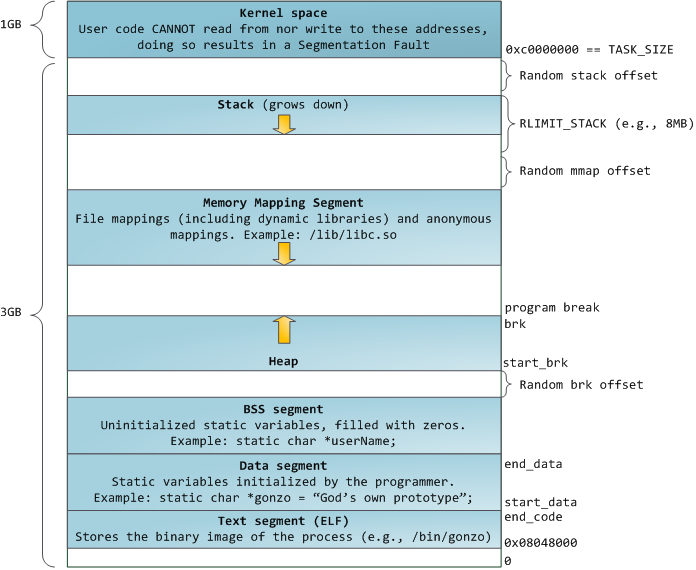
\includegraphics[width=1\columnwidth]{linuxFlexibleAddressSpaceLayout}
	\captionsource{Concept de l'address space layout randomization sous Linux en 32 bits}
	{Concept de l'address space layout randomization sous Linux en 32 bits, par G.~Duarte}
	{\url{http://duartes.org/gustavo/blog/post/anatomy-of-a-program-in-memory/}}
	\label{fig:linuxFlexibleAddressSpaceLayout}
\end{figure}

La \autoref{fig:linuxFlexibleAddressSpaceLayout} montre bien qu'en 32~bits, l'espace disponible n'est au total que de 4~Go, la part d'aléatoire est donc restreinte. À contrario, dans le cas d'un OS 64~bits \gls{aslr} devient bien plus intéressant, car l'espace mémoire virtuel est beaucoup plus vaste (256~To) sans que l'utilisation de celle-ci ne grandisse proportionnellement (au maximum 256~Go de mémoire sont affectés dans des cas classiques d'utilisation serveur). Il donc possible de décaler les segments de manière significative.

Malgré cela, les chercheurs Hector Marco-Gisbert et Ismael Ripoll de l'université de Valence ont écrit un papier démontrant une faiblesse d'\gls{aslr} en 64~bits sous certaines hypothèses \cite{EffectivenessFullASLR64bit}.

\subsection{Limitation et contournements}

Sur un OS 32 bits, la marge de manoeuvre laissée au décalage n'est pas très grande. Seule une partie des bits de l'adresse mémoire est utilisée, ce qui laisse possible à une attaque par recherche exaustive, exigeant quelques milliers d'essais seulement, d'aboutir. En effet la pile est placée aléatoirement avec une entropie de 19 bits seulement et le segment de \og memory mapping \fg avec 8~bits.

L'exemple \autoref{lst:bruteforce_aslr} montre comment avec un code Python d'une trentaine de lignes il est possible de faire une recherche exhaustive en 32 bits et d'exécuter un \og shellcode \fg dans un programme n'utilisant pas \gls{dep}/\gls{nx} et les \og \gls{stackCookies} \fg.

\begin{listing}
	\pythonfile{02-main/listings/aslrBruteforce.py}
	\caption{Exemple de recherche exhaustive en Python sur ASRL en 32 bits}
	\label{lst:bruteforce_aslr}
\end{listing}

Ce code est tiré du blog \og Sirius CTF \fg \cite{ExploitingSimpleBufferOverflow} et illustre l'utilisation de l'opération \mintinline{python}{"\x90"} indiquant au processeur de passer à l'instruction suivante. En définissant une taille de 4096 octets de \og \gls{nop} \fg on augmente drastiquement les chances de tomber sur le \og shellcode \fg. La \autoref{fig:bufferOverflowExploit} montre également l'état de la pile lors d'un dépassement de tampon avec utilisation de l'instruction \gls{nop}.

Le but premier d'\gls{aslr} est de venir contrer la prédictivité de l'emplacement des segments. On constate cependant que sur la \autoref{fig:linuxFlexibleAddressSpaceLayout}, aucun décalage n'est appliqué au segments \og BSS \fg, \og data \fg et \og text \fg, ce qui est tout à fait normal, \gls{aslr} ne modifie pas le segment \og text \fg. Malheureusement cela laisse la prédictibilité de l'emplacement du code exécutable et ouvre la porte à de nouvelles attaques, par exemple de type \og \gls{rop} \fg. Il existe d'autres mécanismes, tel que \og \gls{pie} \fg \cite{PositionIndependentExecutables}, vennant appliquer de l'aléatoire sur certaines partie du code et des bibliothèques. Mais ces mécanismes ne sont pas décrit dans ce rapport.

\vfill

% ---------------------------------------------------------------------------
\section{\og Stack canaries \fg}

Les \og \gls{stackCanaries} \fg ou \og \gls{stackCookies} \fg sont des valeurs déposées sur la pile d'exécution, après la valeur de retour, lors de l'appel d'une fonction. Le nom \og canaries \fg vient par analogie aux canaris que l'on plaçait dans le mine pour prévenir les fuites de monoxyde de carbone \cite{StackCanaries, SentinelSpecies}. Ces oiseaux étant petits et vite atteints par les effets du gaz, ils donnaient rapidement l'informations aux mineurs qu'un danger était présent.

Le fonctionnement des \og \gls{stackCanaries} \fg est pareil, la valeur du canari est vérifiée lors de l'épilogue de la function et, si celle-ci ne correspond pas à la valeur du canari d'origine, alors une tentative de dérouter le flot de contrôle de l'application est détectée et l'on peut alors réagir en conséquence \cite{EpiloguesCanariesBufferOverflows}.

\begin{figure}[H]
	\centering
	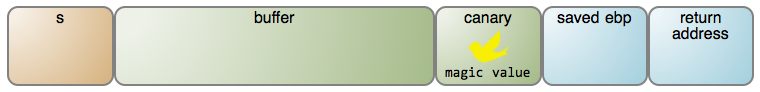
\includegraphics[width=1\columnwidth]{bufferCanary}
	\captionsource{Illustration de l'état de la pile protégée par un canari}
	{Illustration de l'état de la pile protégée par un canari, par G.~Duarte}
	{\url{http://duartes.org/gustavo/blog/post/epilogues-canaries-buffer-overflows/}}
	\label{fig:bufferCanary}
\end{figure}

\subsection{Implémentation}

Il existe trois types principaux de canaris: \og \textit{terminator} \fg, \og \textit{random} \fg, et \og \textit{random XOR} \fg \cite{BufferOverflowProtection}. Les \og \textit{terminator canaries} \fg se base sur le constat que l'exploitation d'un dépassement de tampon est une opération sur une chaîne de caractères. De ce fait, si le canari est constitué de caractères tels que \mintinline{c}{null}, \mintinline{c}{CR}, \mintinline{c}{LF} ou encore \mintinline{c}{-1}, alors la fonction \mintinline{c}{strcpy()} ou \mintinline{c}{gets()} se terminera avant de réécrire l'adresse de retour. Le désavantage notable de cette méthode se retrouve dans le fait que l'attaquant connaît la valeur du canari.

Le \og \textit{random canary} \fg est tiré aléatoirement afin de palier au problème du \og \textit{terminator canary} \fg. Généralement ce canari est généré à l'initialisation du programme et est stocké dans une variable globale.

Le \og \textit{random XOR canary} \fg est une méthode un peu plus élaborée, elle fonctionne de la même manière que le \og \textit{random canary} \fg mais est en plus calculée en fonction de tout ou partie du programme, ce qui rend encore plus difficile pour l'attaquant de forger un canari valide.

L'application de la protection par canaries au sein de \gls{clang}/\gls{llvm} peut se faire grâce au composant \og StackProtector \fg \cite{LLVMStackProtector}. Ce composant effectue une analyse lors de la compilation, couplée à l'utilisation d'une librairie lors de l'exécution.

\subsection{Limitation et contournements}

Dans les deux premières implémentations --- \og \textit{terminator canaries} \fg et \og \textit{random canaries} \fg ---, il est possible de contourner les canaris en récupérant leur valeur. Ce qui peut être fait directement sur la pile d'exécution grâce au contrôle, par exemple, des paramètres d'une fonction tel que \mintinline{c}{printf()} qui nous permet de lire en mémoire grâce au format \mintinline{c}{%p}.

Dans le cas d'un \og \textit{random XOR canary} \fg, si l'adresse de retour est modifiée, alors la valeur du canari change, car elle dépend de la valeur aléatoire de départ et des données sur la pile d'exécution. L'exploitation devient alors plus complexe à mettre en place mais reste possible.

% ---------------------------------------------------------------------------
\section{\og Control-flow integrity \fg}

\gls{cfi} est un concept permettant, par analyse statique, de définir les changements possibles du flot de contrôle de l'application, appelé \og \gls{cfg} \fg, pour ensuite valider ou non le changement effectif lors de l'exécution du programme. Le papier original démontrant l'approche \cite{CFIPaper}, publié en 2005, est généralement attribué au centre de recherche de Microsoft. Depuis, de nombreux papiers ont été publiés améliorant les performances ou modifiant légèrement l'approche.

Actuellement le concept de \gls{cfi} est implémenté au sein de \gls{clang} sous le nom de \og forward-edge CFI \fg \cite{ControlFlowIntegrity, TalkAboutCFIClang, ControlFlowIntegrityDesignDocumentation}. Dans la documentation dédiée, un example de coût en performance de 15\% est relevé sur Chromium. On peut également constater, dans d'autre sources de la litérature, que l'approche classique impose un coût de 16\% en moyenne et de 45\% dans le pire des cas \cite{ControlFlowIntegrityMaryland}. Ce qui en fait la principale faiblesse de cette approche.

Les principales variations du concept se font sur la granularité choisie lors de la construction du \gls{cfg}. Deux \og modèles \fg émèrgent et se généralisent: \og \gls{fg-cfi} \fg et \og \gls{cg-cfi} \fg.

\subsection{\og Fine-grained CFI \fg}

La variation \og \gls{fg-cfi} \fg \cite{FineCFI, FineCFIKernel}, comme son nom l'indique, a une approche précise lors de la construction du \gls{cfg}. Chaque élément du graphe est labélisé de manière précise et lors de l'exécution du programme, à chaque changement du flot de contrôle on vérifie si la destination labélisée correspond à un label voisin de l'élément de départ. Cependant cette manière de faire amène, par ces nombreuses vérifications, un coût important en terme de performances.

\subsection{\og Coarse-grained CFI \fg}

La variation \og \gls{cg-cfi} \fg est une approche plus simple quant à la labélisation du \gls{cfg},  et donc plus performante, mais ouvrant la porte à certaines faiblesses. Les points de contrôle de l'application son labélisés de manière à obtenir un nombre restreint de labels. Ceux-ci sont alors réutilisés au sein du même graphe, de ce fait il est possible de partir d'un point A et aller au point C alors que cela n'est pas prévu, mais par cause d'une labélisation non unique l'erreur n'est pas détectée.

\newpage

\section{Résumé}

Il existe à ce jour une multitude de concepts ayant pour mission d'entraver ou de ralentir les attaques visant le flot de contrôle d'une application. Ces concepts ne gèrent, individuellement, qu'une partie de la problématique et sont donc généralement appliqués conjointement. Aujourd'hui, il n'existe pas encore de mécanismes permettant de garantir seul, à 100\%, l'intégrité du flot sans engager des coûts trop importants en performance, rendant leur utilisation impossible dans un environnement de production. Tous les mécanismes de protection passés en revue peuvent être contourné par une attaque évoluée de type \gls{rop}.

Le papier présentant CPI/CPS/SafeStack \cite{CPIPaper} et son prototype appelé \gls{levee} promettent un mécanisme permettant de contrer ce type d'attaque et à moindre coût. Afin d'y parvenir, l'équipe de chercheurs à mis en place différents concepts se raprochant de ce qui se fait au sein des languages de programmation de type \og memory-safe \fg. En effet, les implémentations actuelles permettant de garantire à 100\% le flot de contrôle --- SoftBound+CETS, CCured ou encore AddressSanitizer --- sont une application directe des concepts présent au sein des languages de type \og memory-safe \fg aux languages C/C++. Cependant cette application directe n'est pas viable en terme de performances. Les chercheurs du projet \gls{levee} ont alors proposé d'appliquer ces méthodes sur une partie spécifique du programme.

% \newpage

% % -------------------------------------------------------------------------
% This chapter shows example of picture and also serves to populate the different lists: list of figures, list of tables, bibliography, and glossary.
%
% \section{Tables}
%
% This section contains an examples of table: \autoref{tab:esempio}
%
% \begin{table}[H]
% 	\centering
% 	\begin{tabular}{ccc}
% 		\toprule
% 		name & weight & food \\
% 		\midrule
% 		mouse	& 10 g	& cheese \\
% 		cat	& 1 kg	& mice \\
% 		dog	& 10 kg	& cats \\
% 		t-rex	& 10 Mg	& dogs \\
% 		\bottomrule
% 	\end{tabular}
% 	\caption[A floating table]{A floating table.}
% 	\label{tab:esempio}
% \end{table}
%
% \section{Figures}
%
% This section contains examples of figures: \autoref{fig:galleria}, \autoref{fig:lorem}, \autoref{fig:ipsum}, \autoref{fig:dolor}, \autoref{fig:sit}
%
% \begin{figure}[H]
% 	\centering
% 	\includegraphics[width=0.5\columnwidth]{galleria_stampe}
% 	\captionsource{A floating figure}{A floating figure: the lithograph \emph{Galleria di stampe}, of M.~Escher}{\url{http://www.mcescher.com/}}
% 	\label{fig:galleria}
% \end{figure}
%
% \begin{figure}[H]
% 	\centering
% 	\begin{subfigure}[b]{0.45\textwidth}
% 		\includegraphics[width=\textwidth]{lorem}
% 		\caption{A gull}
% 		\label{fig:lorem}
% 	\end{subfigure}
% 	~ %add desired spacing between images, e. g. ~, \quad, \qquad, \hfill etc.
% 	%(or a blank line to force the subfigure onto a new line)
% 	\begin{subfigure}[b]{0.45\textwidth}
% 		\includegraphics[width=\textwidth]{ipsum}
% 		\caption{A tiger}
% 		\label{fig:ipsum}
% 	\end{subfigure}
% 	~ %add desired spacing between images, e. g. ~, \quad, \qquad, \hfill etc.
% 	%(or a blank line to force the subfigure onto a new line)
% 	\begin{subfigure}[b]{0.45\textwidth}
% 		\includegraphics[width=\textwidth]{dolor}
% 		\caption{A mouse}
% 		\label{fig:dolor}
% 	\end{subfigure}
% 	~ %add desired spacing between images, e. g. ~, \quad, \qquad, \hfill etc.
% 	%(or a blank line to force the subfigure onto a new line)
% 	\begin{subfigure}[b]{0.45\textwidth}
% 		\includegraphics[width=\textwidth]{sit}
% 		\caption{A mouse}
% 		\label{fig:sit}
% 	\end{subfigure}
% 	\caption{Example subcaption}\label{fig:animals}
% \end{figure}
%
%
% % -----------------------------------------------------------------------------
% \section{Code}
%
% \autoref{lst:listing_example} shows an example of Java code rendered with minted.
%
% \begin{listing}
% 	\javafile{02-main/listings/HelloWorld.java}
% 	\caption{Example of listing using the minted package}
% 	\label{lst:listing_example}
% \end{listing}
%
% % -----------------------------------------------------------------------------
% \section{Other features}
%
% Term (glossaries): \gls{nosql}
%
% Acronym (glossaries): \gls{sql}
%
% Citation (biblatex): \cite{paper_millwheel}
%
% % -----------------------------------------------------------------------------
% \section{Conclusion}
%
% \blindtext
